\documentclass[a4paper,12pt,oneside]{book}

%-------------------------------Start of the Preable------------------------------------------------
\usepackage[english]{babel}
\usepackage{blindtext}
%packagr for hyperlinks
\usepackage{hyperref}
\hypersetup{
    colorlinks=true,
    linkcolor=blue,
    filecolor=magenta,      
    urlcolor=cyan,
}

\urlstyle{same}
%use of package fancy header
\usepackage{fancyhdr}
\setlength\headheight{26pt}
\fancyhf{}
%\rhead{
\includegraphics[width=1cm]{logo}}
%\lhead{\rightmark}
%\rhead{
\includegraphics[width=1cm]{logo}}
\fancyfoot[RE, RO]{\thepage}
\fancyfoot[CE, CO]{\href{http://www.e-yantra.org}{www.e-yantra.org}}

\pagestyle{fancy}

%use of package for section title formatting
\usepackage{titlesec}
\titleformat{\chapter}
  {\Large\bfseries} % format
  {}                % label
  {0pt}             % sep
  {\huge}           % before-code
 
%use of package tcolorbox for colorful textbox
\usepackage[most]{tcolorbox}
\tcbset{colback=cyan!5!white,colframe=cyan!75!black,halign title = flush center}

\newtcolorbox{mybox}[1]{colback=cyan!5!white,
colframe=cyan!75!black,fonttitle=\bfseries,
title=\textbf{\Large{#1}}}

%use of package marginnote for notes in margin
\usepackage{marginnote}

%use of packgage watermark for pages
%\usepackage{draftwatermark}
%\SetWatermarkText{
\includegraphics{logo}}
\usepackage[scale=2,opacity=0.1,angle=0]{background}
\backgroundsetup{
contents={
\includegraphics{logo}}
}

%use of newcommand for keywords color
\usepackage{xcolor}
\newcommand{\keyword}[1]{\textcolor{red}{\textbf{#1}}}

%package for inserting pictures
\usepackage{graphicx}

%package for highlighting
\usepackage{color,soul}

%new command for table
\newcommand{\head}[1]{\textnormal{\textbf{#1}}}


%----------------------End of the Preamble---------------------------------------


\begin{document}

%---------------------Title Page------------------------------------------------
\begin{titlepage}
\raggedright
{\Large eYSIP2016\\[1cm]}
{\Huge\scshape Farm Produce: Logging And Monitoring \\[.1in]}
\vfill
\begin{flushright}
{\large Bhavesh Jadav \\}
{\large Ankur Panwar \\}
{\large MENTORS\hspace{.1in}:}
{\large Saurav Shandilya\\}
{\large Parin Chheda\\}
{\Large Vishwanathan\\}
{\large Duration of Internship: $ 27/05/2016-10/07/2016 $ \\}
\end{flushright}

{\itshape 2016, e-Yantra Publication}
\end{titlepage}
%-------------------------------------------------------------------------------

\chapter[Project Tag]{Farm Produce: Logging And \\ Monitoring}
\section*{Abstract}
This project logs crop data in a green house to reduce manual labour. Essentially, it is a weighing machine connected to Internet.\\
A weighing machine will be delivered to user which can measure weight of crop by using load cell. User can input information related to crop via keypad. User will be assisted by continuous messages on screen. After successful data entry the data will automatically pushed to database. Local people can also take advantage of crop production by placing order through e-commerce website after filling details.

\subsection*{Completion Status}
The project is successfully completed providing "weighing platform, screen, keypad, e-commerce website, admin-panel and user manual." 

\section{Hardware Parts}
\begin{itemize}
  \item Hardware parts
    \begin{itemize}
      \item Load cell
      \item 20x4 LCD
      \item 4x4 Keypad
      \item Raspberry pi 2 Model B
      \item LM2596 step-down voltage regulator
      \item HX711(ADC amplifier)
      \item USB Camera
      \item DC Adapter
      \item Enclosure to hold all parts
    \end{itemize}
  \item Detail of each hardware:\\
    \href{https://cdn.sparkfun.com/datasheets/Sensors/ForceFlex/hx711_english.pdf}{HX711 ADC Amplifier}\\
    \href{http://www.kadcontrols.com/KadWebsite/LoadCell_Tech/CZL601.pdf}{Load cell CZL601}\\
    \href{http://www.onsemi.com/pub_link/Collateral/LM2596-D.PDF}{Step down voltage regulator}\\
    \href{http://lispol.com/uploaded/products_files/1364491305_79923300.pdf}{20x4 LCD}\\
    \href{https://www.parallax.com/sites/default/files/downloads/27899-4x4-Matrix-Membrane-Keypad-v1.2.p    df}{Membrane Keypad}\\
     \href{https://cdn-shop.adafruit.com/pdfs/raspberrypi2modelb.pdf}{Raspberry pi 2 Model B}\\
     \href{https://www.parallax.com/sites/default/files/downloads/27899-4x4-Matrix-Membrane-Keypad-v1.2.pdf}{4x4 Keypad}\\
  
\end{itemize}

\section{Software Used}
\begin{itemize}
   \item List of software used
  \begin{itemize}
   \item  win32 disk imager
   \item  Raspbian wheezy
   \item Notepad++
   \item Local server(xampp apache)
   \item Mysql(xampp)
   \item Diptrace
   \item Corel draw
   \item Autodesk Autocad
   \item Solidworks
   \item Atom text editor
   \item Opencart framework
  \end{itemize}
\end{itemize} 
\begin{itemize}
   \item link of software: \\
  \href{https://sourceforge.net/projects/win32diskimager/}{win32 disk imager}\\
  \href{https://www.raspberrypi.org/downloads/}{Raspbian OS}\\
  \href{https://www.apachefriends.org/download.html}{Xampp}\\
  \href{https://notepad-plus-plus.org/download/v6.9.2.html}{Notepad++}\\
  \href{http://diptrace.com/download-diptrace/}{Diptrace}
\end{itemize}

\section{Assembly Of Hardware}
\subsection*{Dimensions Of Enclosure}
\begin{figure}[!htb]
\minipage{0.24\textwidth}
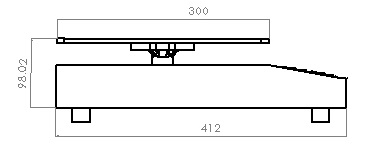
\includegraphics[width=\linewidth]{d1.jpg}
\caption{Side View}
\endminipage\hfill
\minipage{0.24\textwidth}
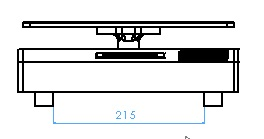
\includegraphics[width=\linewidth]{d2.jpg}
\caption{Front View}
\endminipage\hfill
\minipage{0.24\textwidth}
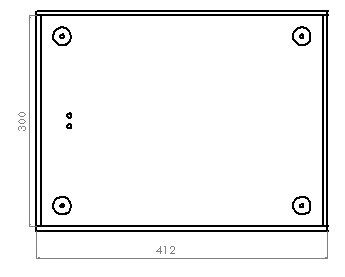
\includegraphics[width=\linewidth]{d3.jpg}
\caption{Bottom View}
\endminipage
\end{figure}}
\begin{figure}[!htb]
\minipage{0.24\textwidth}
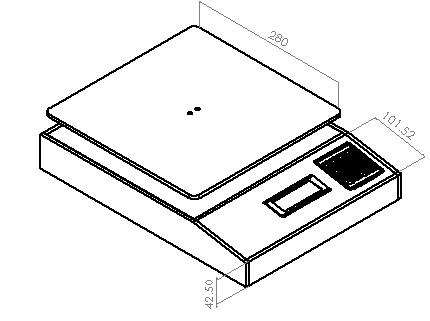
\includegraphics[width=\linewidth]{d4.jpg}
\caption{Isometric View}
\endminipage\hfill
\minipage{0.24\textwidth}
%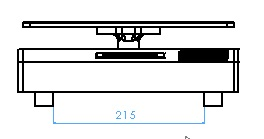
\includegraphics[width=\linewidth]{d2.jpg}
%\caption{Front View}
\endminipage\hfill
\minipage{0.24\textwidth}
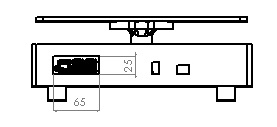
\includegraphics[width=\linewidth]{d5.jpg}
\caption{Back View}
\endminipage
\end{figure}}
\subsection*{Block Diagram}
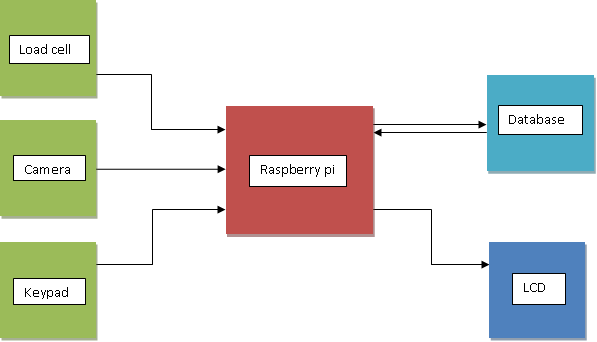
\includegraphics[width=12cm,height=7cm]{chart.png}
\subsection*{Connection Diagram}\\\\
\begin{figure}[!htb]
\minipage{0.24\textwidth}
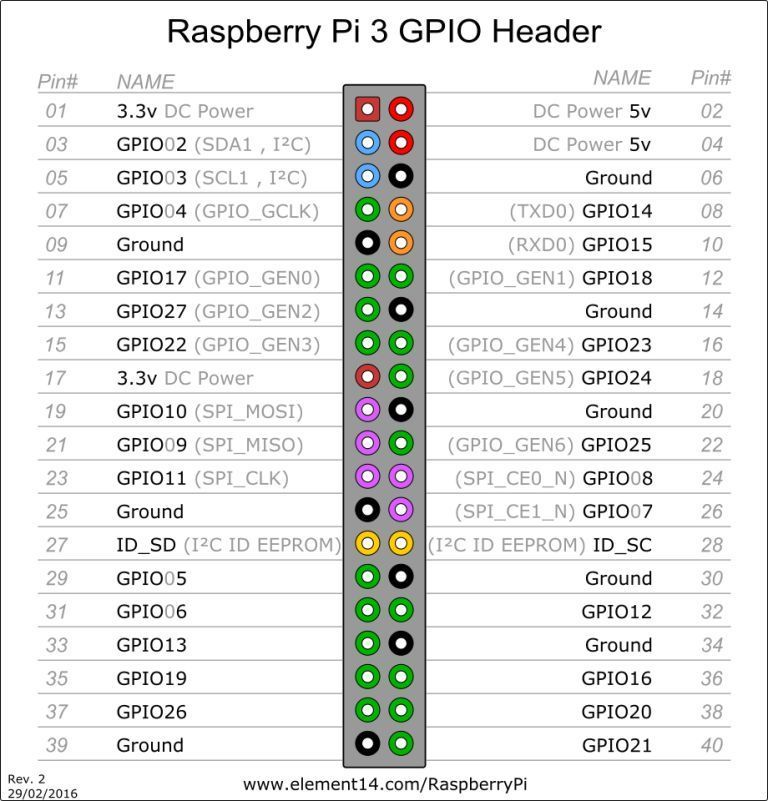
\includegraphics[width=6cm,height=8cm]{pigpio.jpg}
\caption{Rpi pin-out}
\endminipage\hfill
\minipage{0.24\textwidth}
%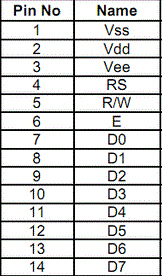
\includegraphics[width=2cm,height=2cm]{lcd.png}
%\caption{LCD pin-out}
\endminipage\hfill
\minipage{0.24\textwidth}
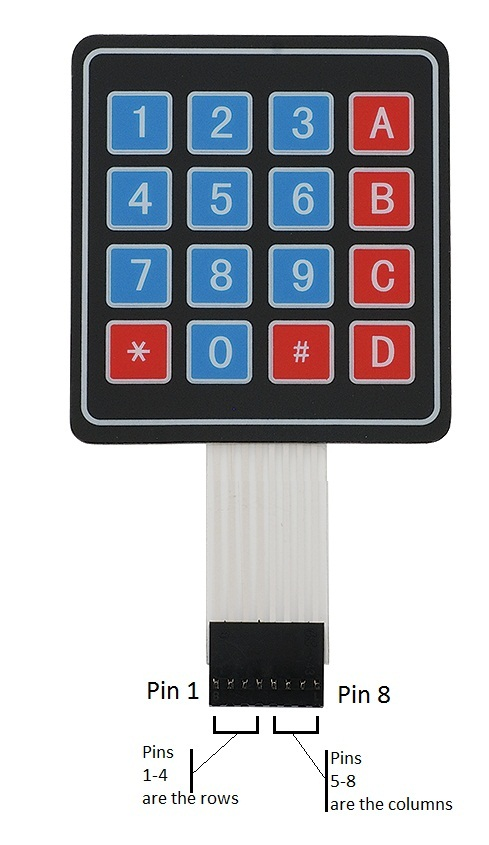
\includegraphics[width=\linewidth]{keypad.jpg}
\caption{Keypad pin-out}
\endminipage
\end{figure}}
%\item Raspberry pi pinout 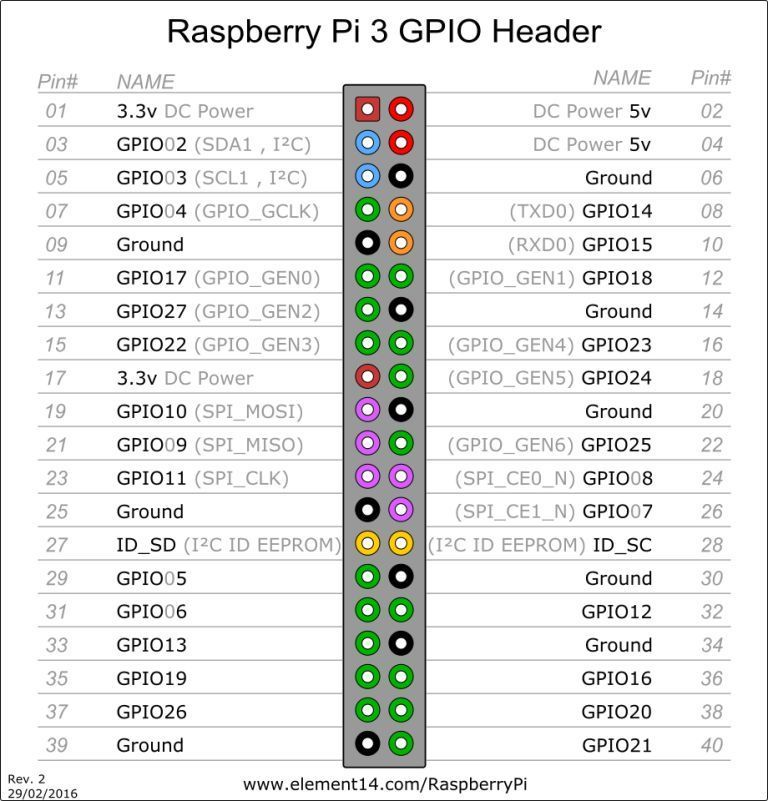
\includegraphics[height=7cm,width=6cm]{pigpio.jpg}\\

\begin{figure}[!htb]
\minipage{0.24\textwidth}
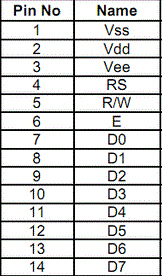
\includegraphics[width=\linewidth]{lcd.png}
\caption{LCD pin-out}
\endminipage\hfill
\minipage{0.24\textwidth}
%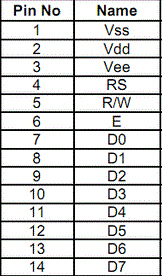
\includegraphics[width=2cm,height=2cm]{lcd.png}
%\caption{LCD pin-out}
\endminipage\hfill
\minipage{0.24\textwidth}
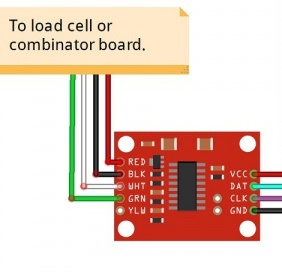
\includegraphics[width=4cm,height=4cm]{loadcell.jpg}
\caption{load cell pin-out}
\endminipage
\end{figure}}

\subsection{Schematic Interface Between Modules}
\begin{figure}[!htb]
\minipage{0.24\textwidth}
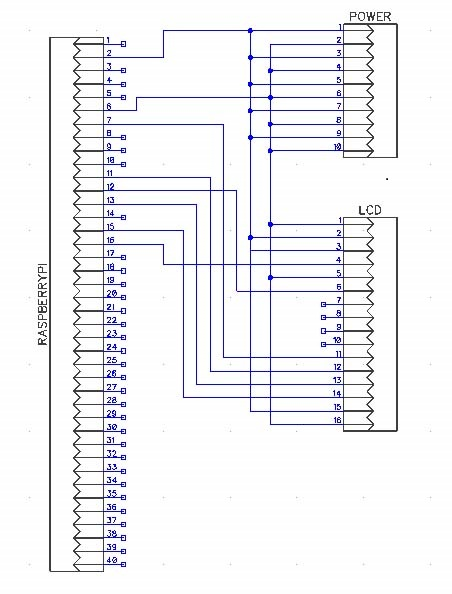
\includegraphics[width=\linewidth]{connection1.jpg}
\caption{Rpi, power and LCD}
\endminipage\hfill
\minipage{0.24\textwidth}
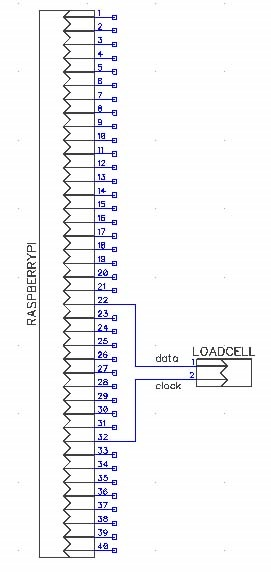
\includegraphics[width=\linewidth]{connection2.jpg}
\caption{Rpi and Load cell}
\endminipage\hfill
\minipage{0.24\textwidth}
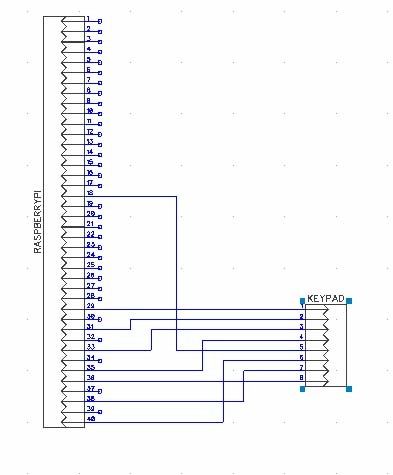
\includegraphics[width=\linewidth]{connection3.jpg}
\caption{Rpi and keypad}
\endminipage
\end{figure}}
%\item Keypad pinout 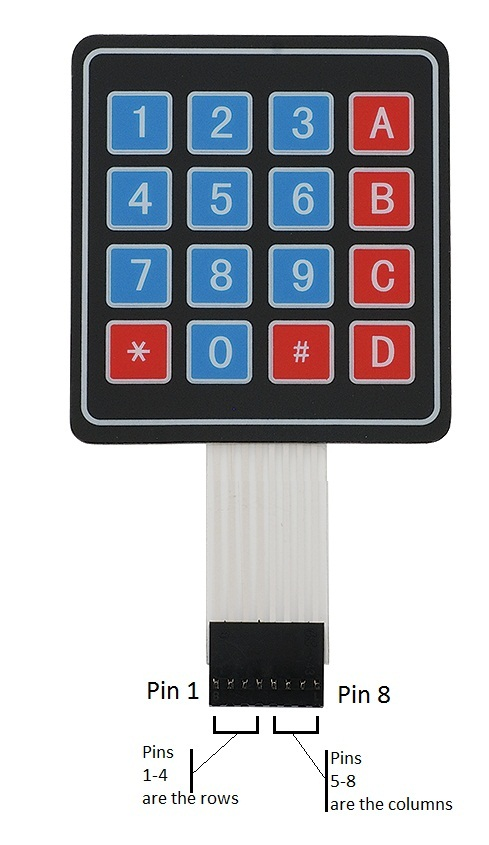
\includegraphics[height=12cm, width=7cm]{keypad.jpg}\\

\section{Software And Code}
\href{https://github.com/eYSIP-2016/eYSIP-2016-Farm-Produce-Logging-and-Monitoring/tree/master}{Github link}\\\\
e-Commerce website\\\\
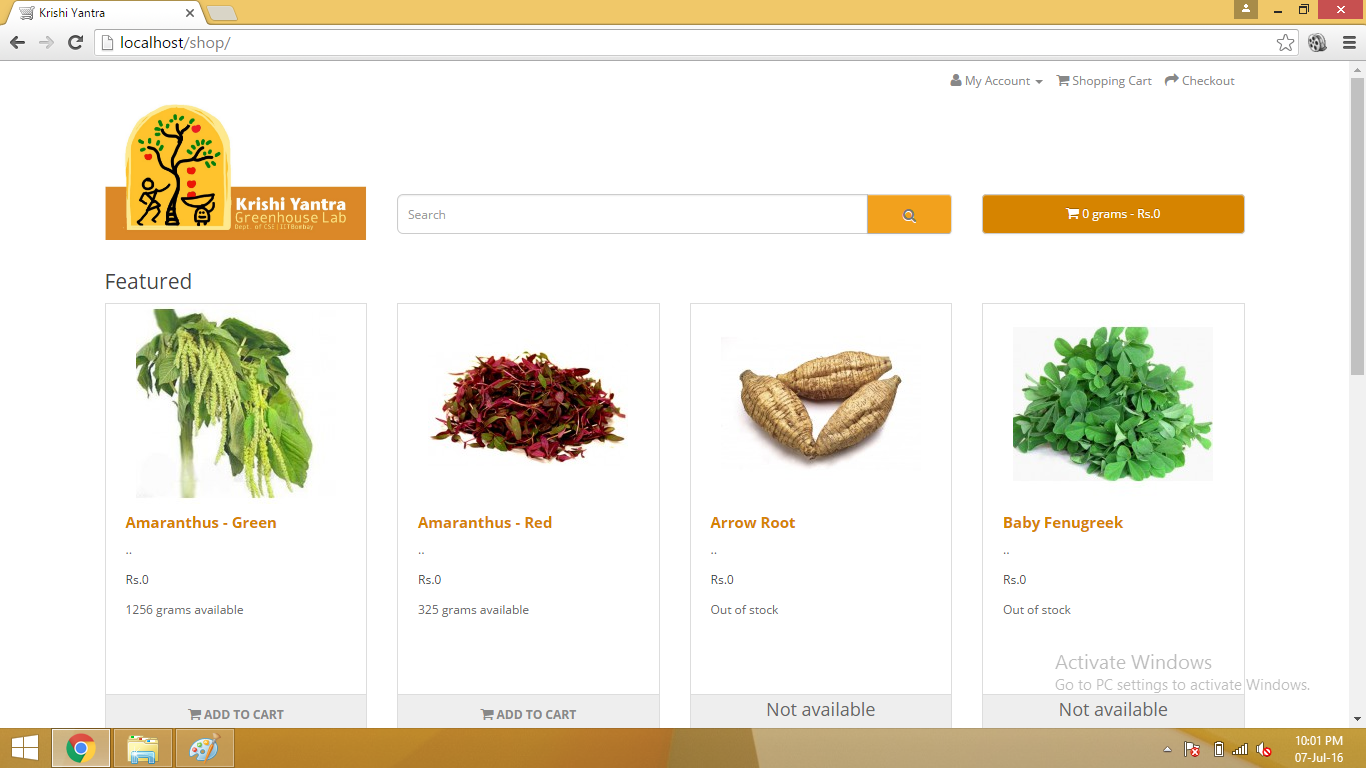
\includegraphics[width=12cm,height=7cm]{page.png}\\

\subsection*{Assembling Steps}
The dimension of the machine is 40x30x11.5cm. More detailed version of model can be found on github.\\\\
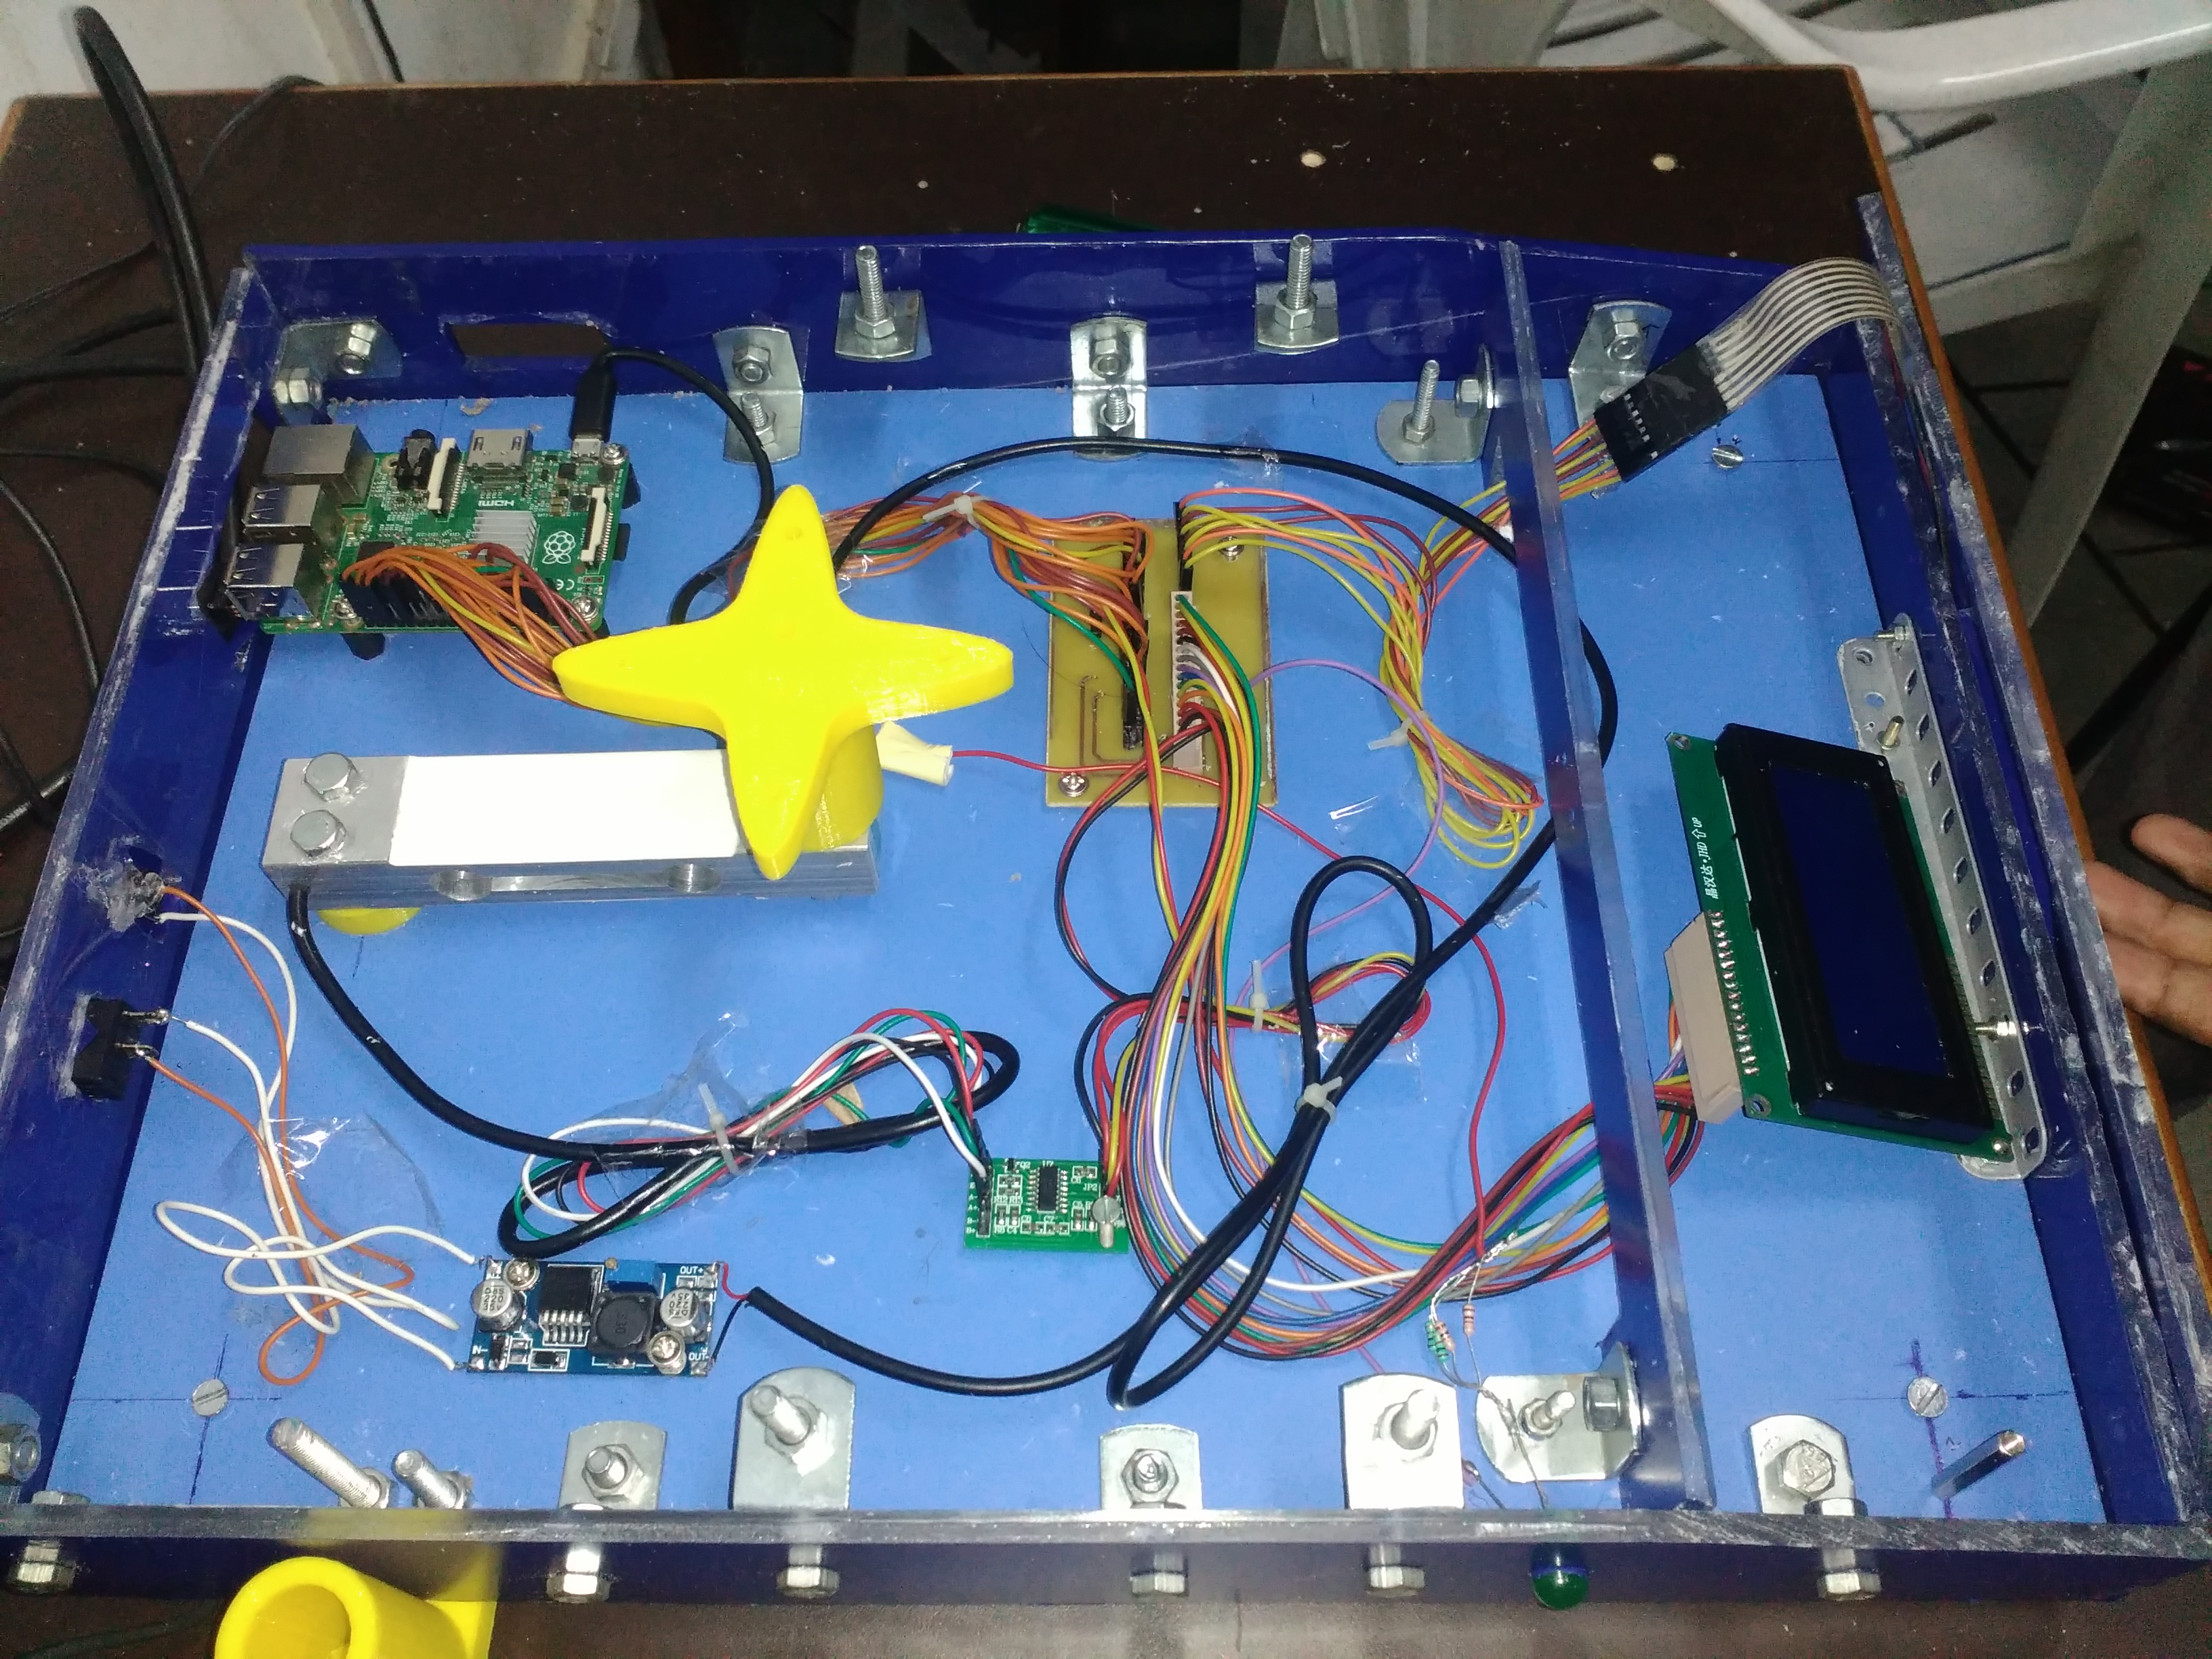
\includegraphics[height=8cm,width=10cm]{1.jpg}\\
Step 1: Attach side plates, front plate, middle plate and back plate by using L clamps as shown in above diagram.\\\\\\
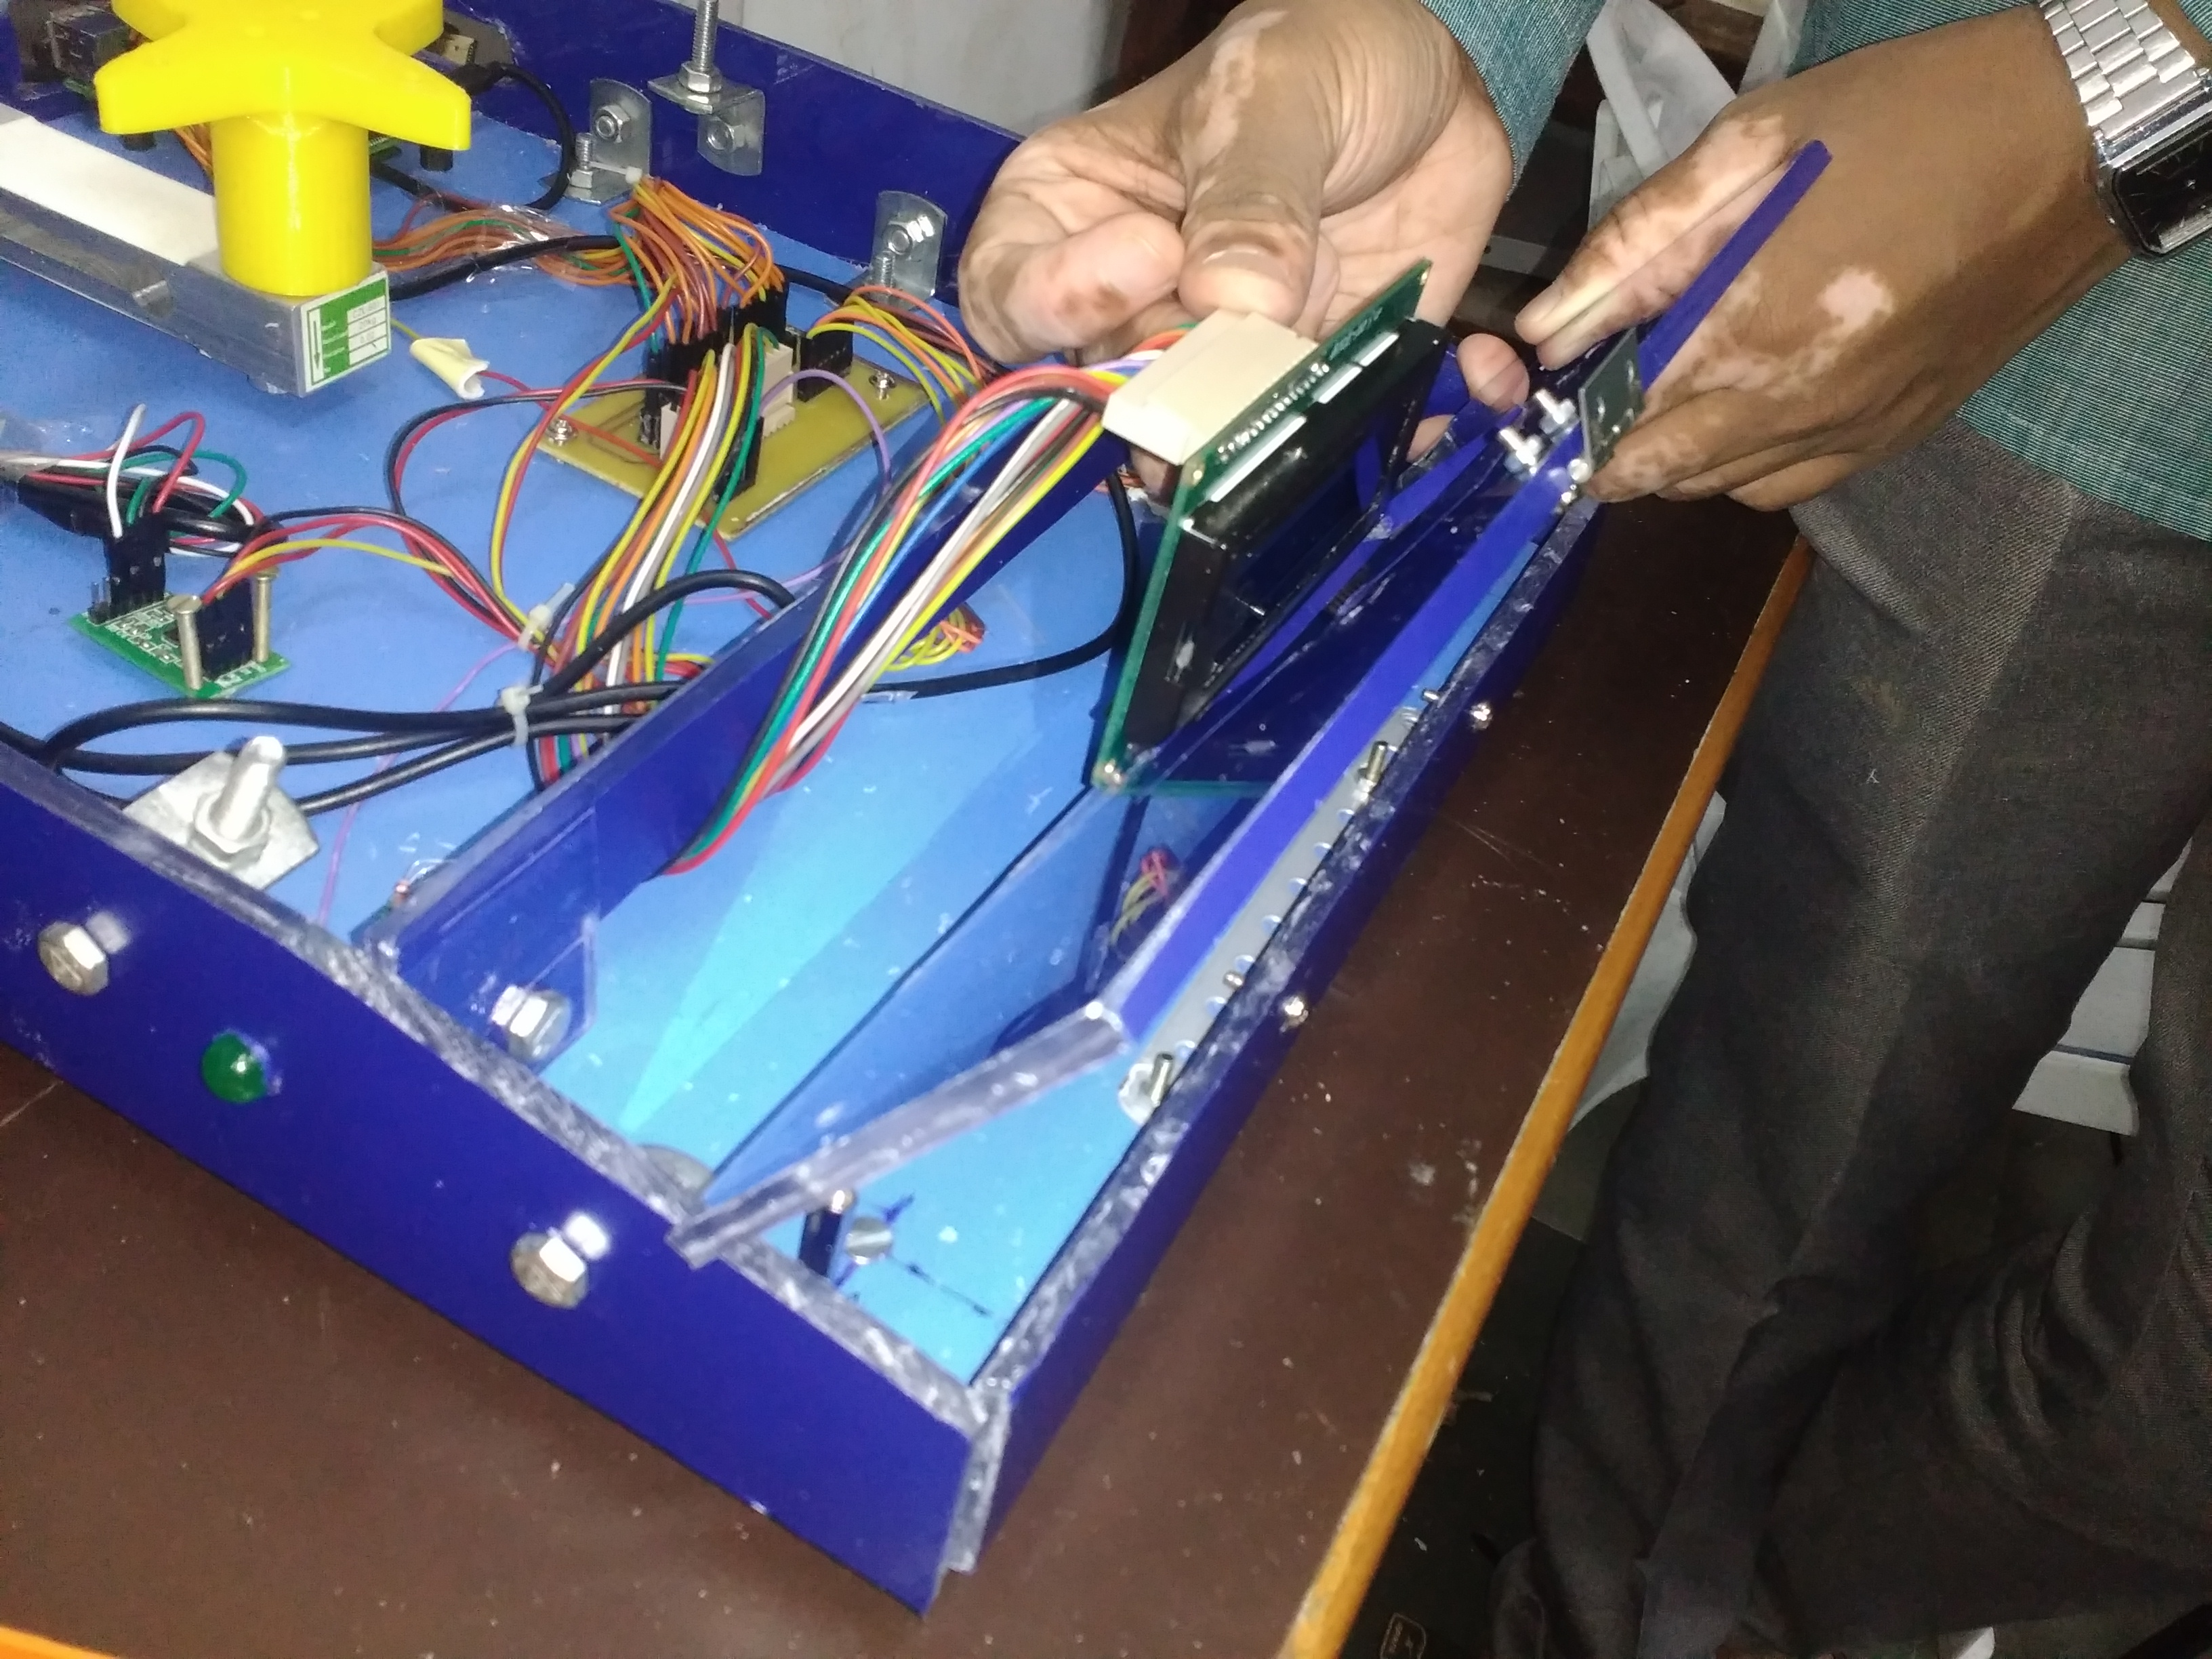
\includegraphics[height=8cm,width=13cm]{2.jpg}\\
Step 2: Place LCD on front panel. Use 20x4 LCD.\\
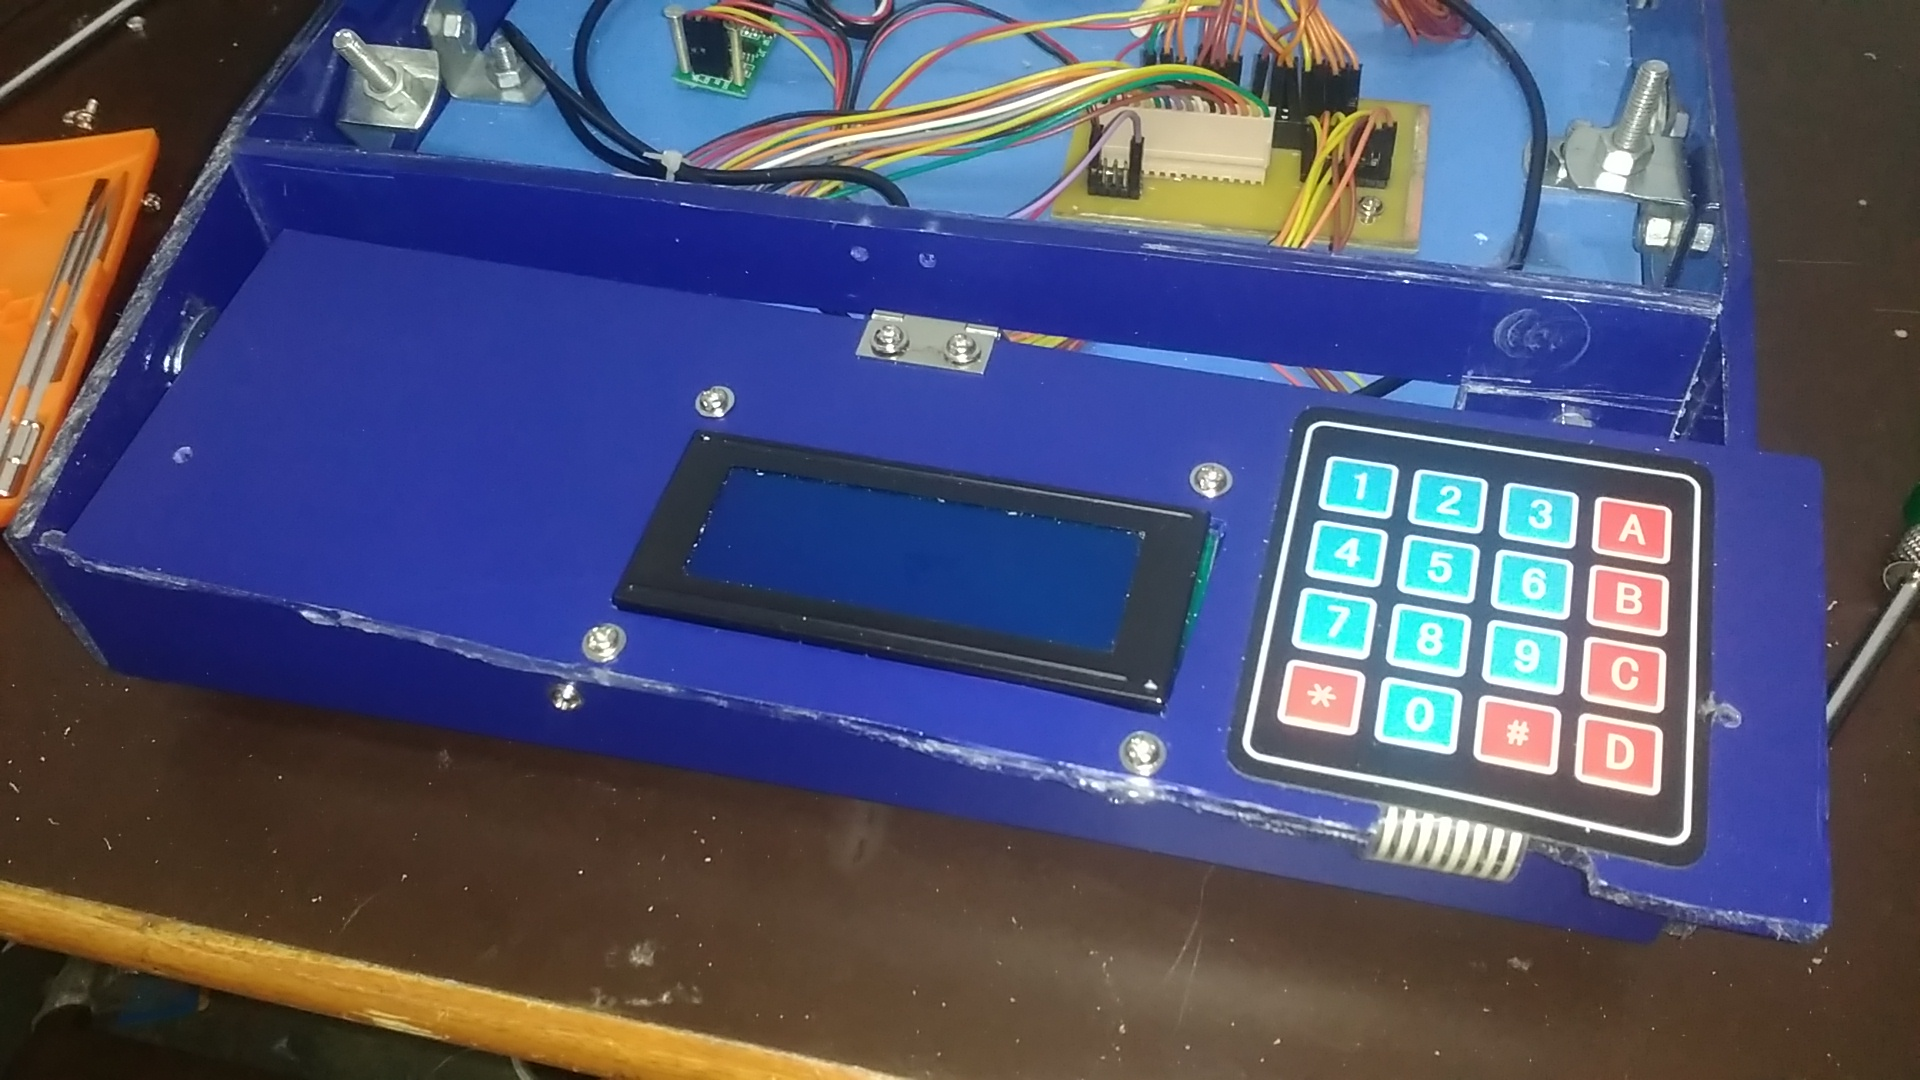
\includegraphics[height=8cm,width=13cm]{3.jpg}\\
Step 3: Use four 3mm screws with bolts to fix the LCD on panel. After attaching LCD, Attach keypad to the front panel\\\\\\
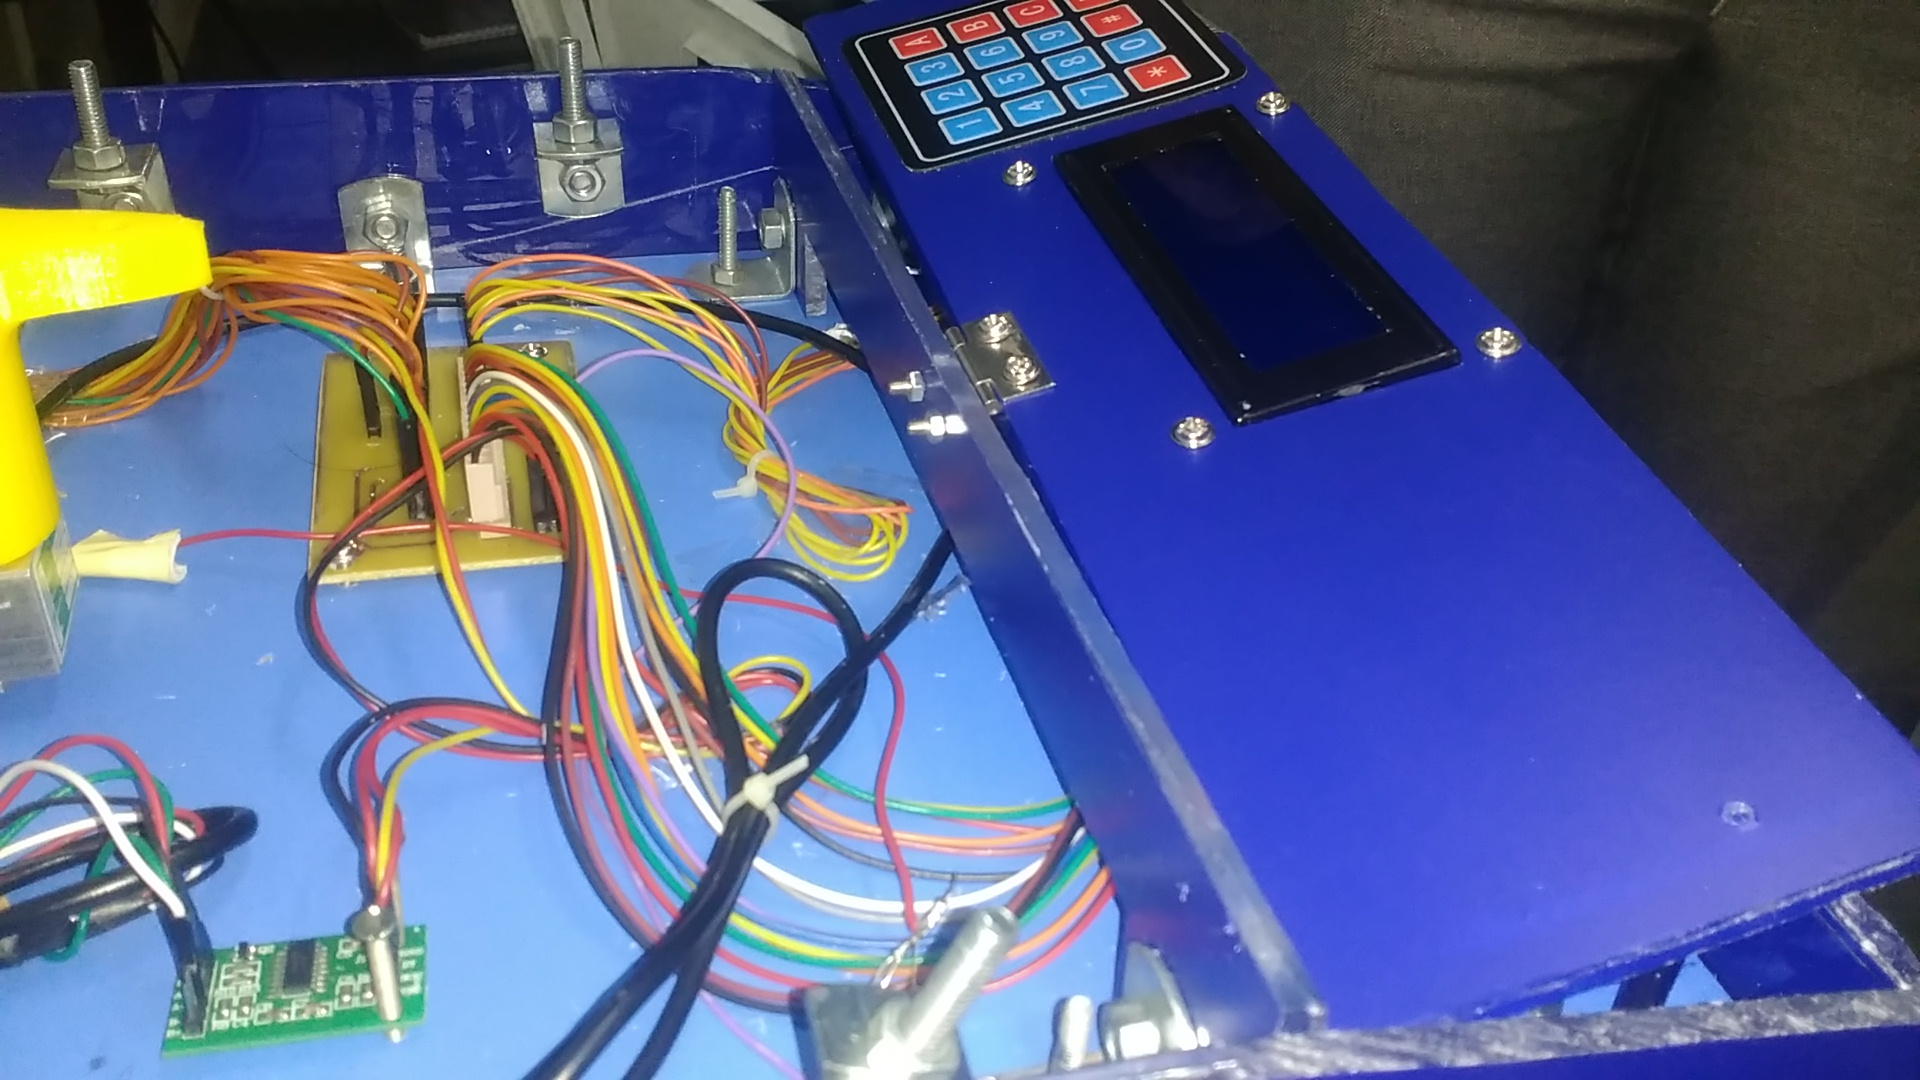
\includegraphics[height=8cm,width=13cm]{4.jpg}\\
Step 4: Attach front panel to the middle plate with the help of hinge. Use 3mm screws with bolts to attach front panel to middle plate.\\
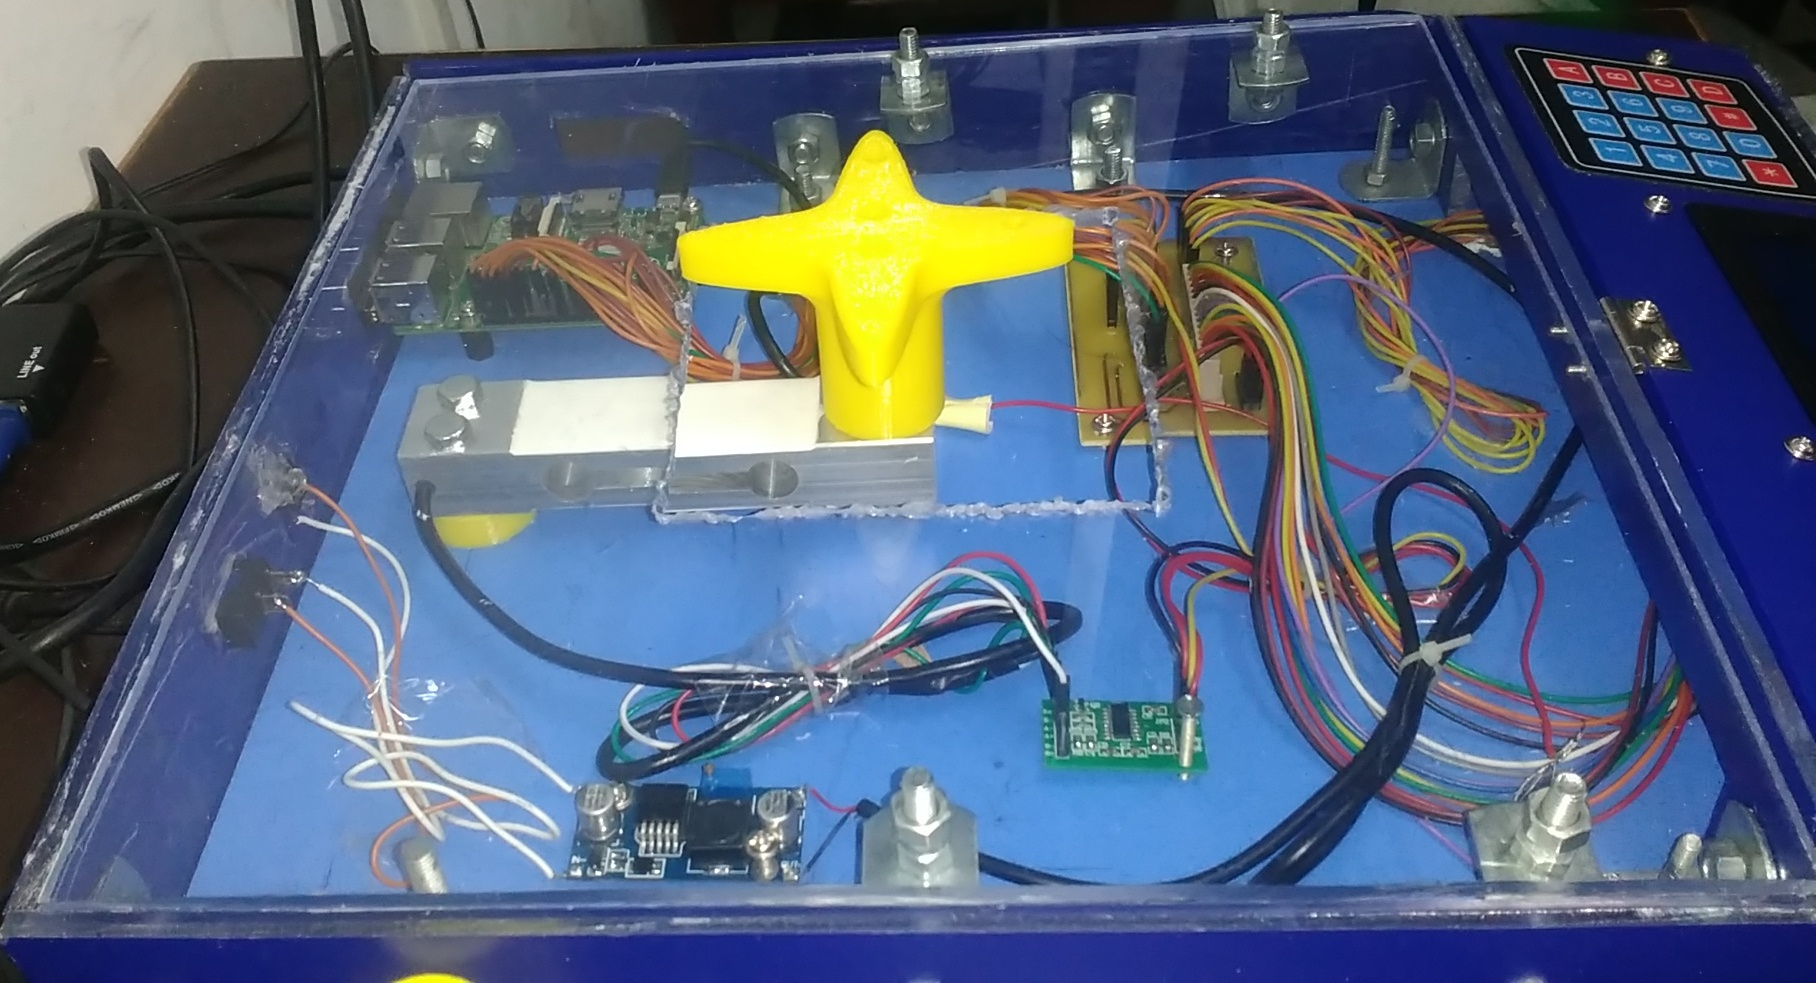
\includegraphics[height=8cm,width=13cm]{5.jpg}\\
Step 5: After attaching front panel, place the second top most plate over 4 screws attached with side plates. After
putting the plate, user four nuts to fix the plate.\\\\\\
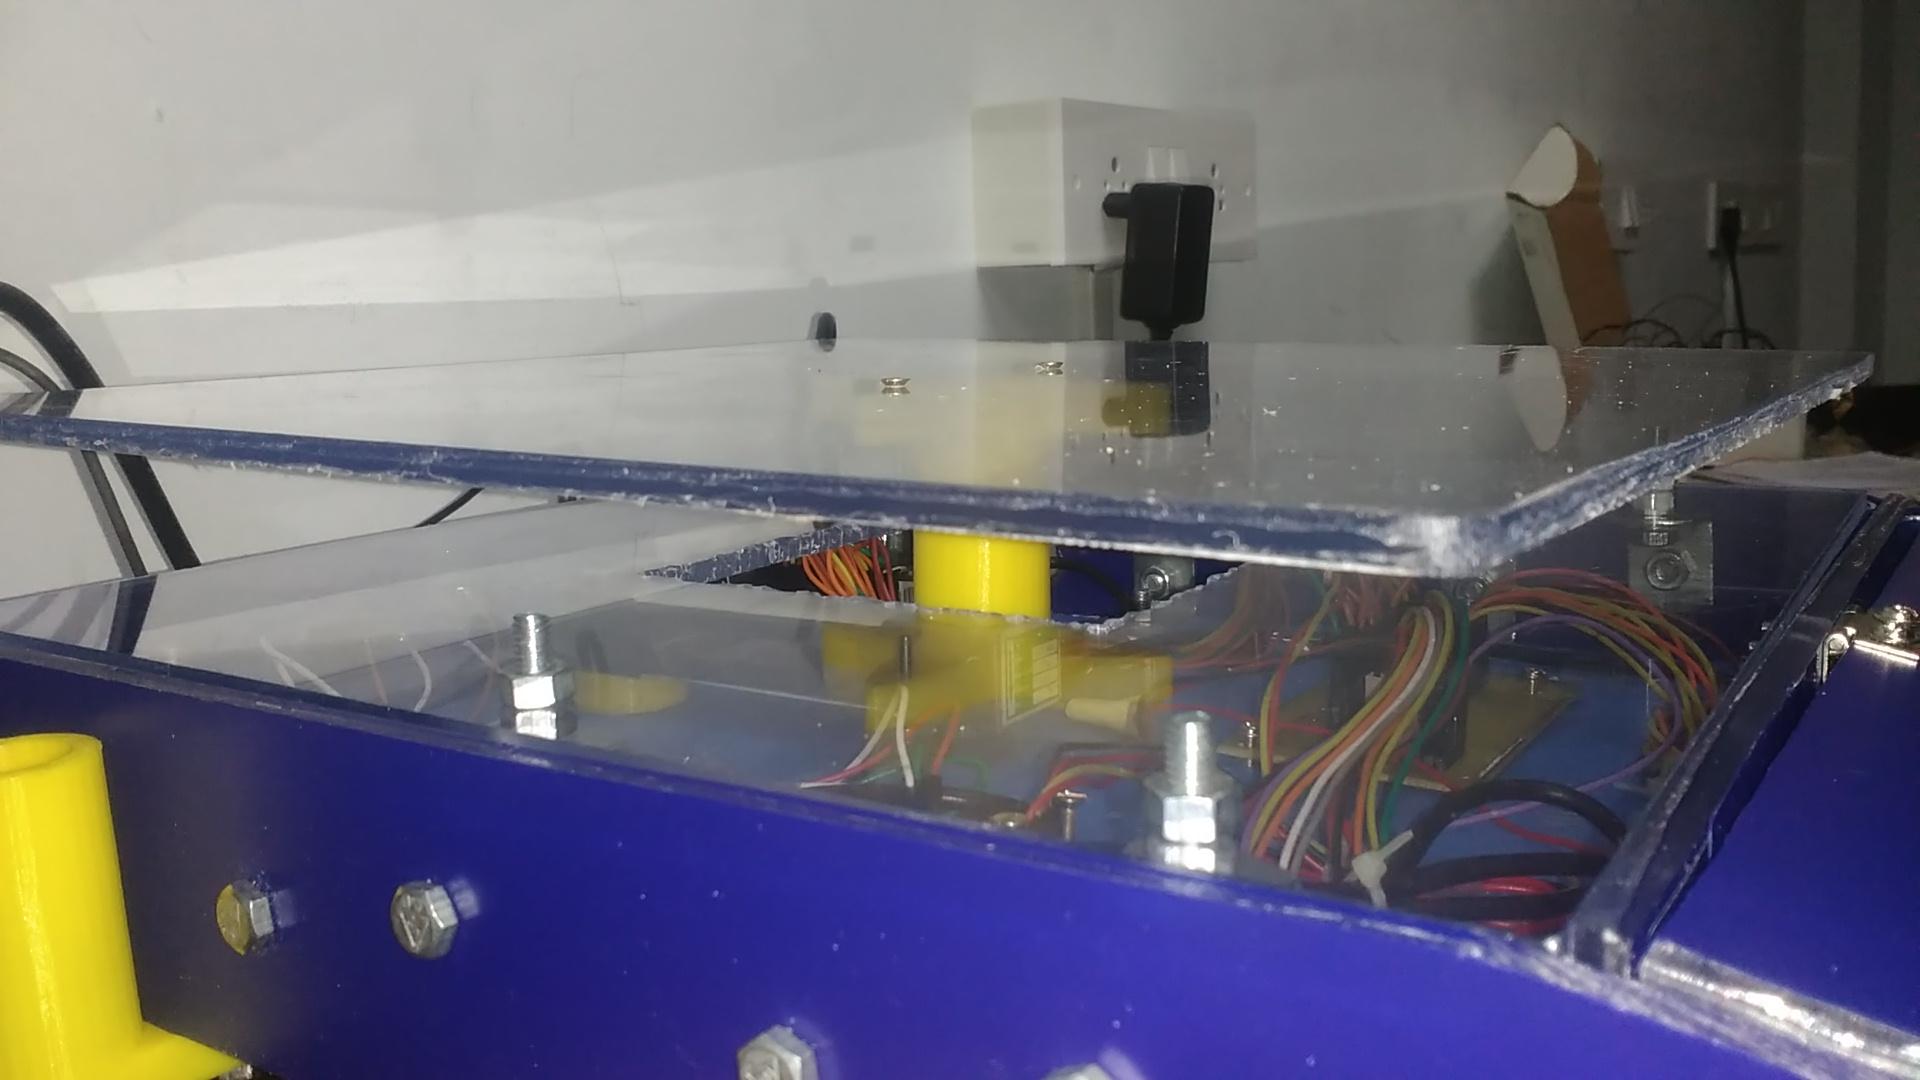
\includegraphics[height=8cm,width=13cm]{6.jpg}\\ 
Step 6: Attach weighing platform on top of star shaped design and use 3mm screws with nuts to fix it.\\
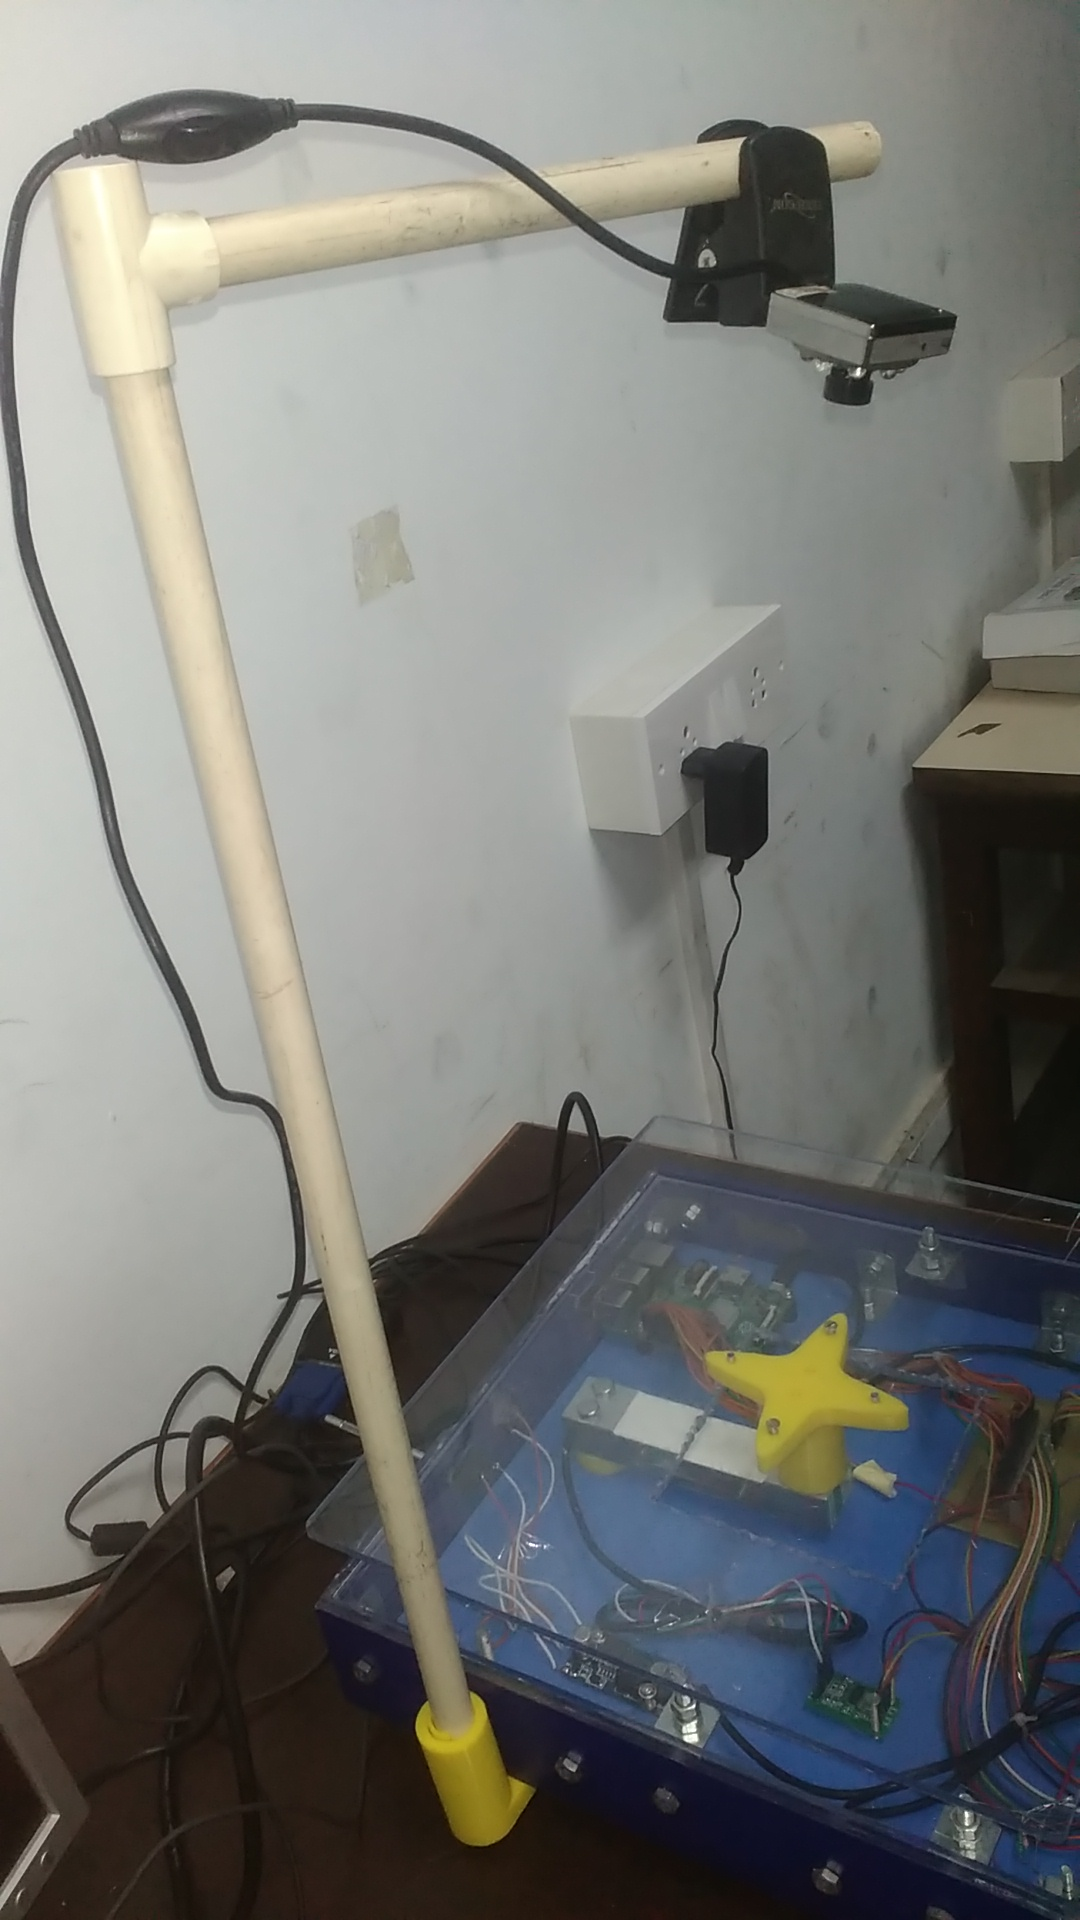
\includegraphics[height=8cm,width=12cm]{7.jpg}\\
Step 7: Finlay attach camera stand at side of the machine.\\



\section{Final Product}
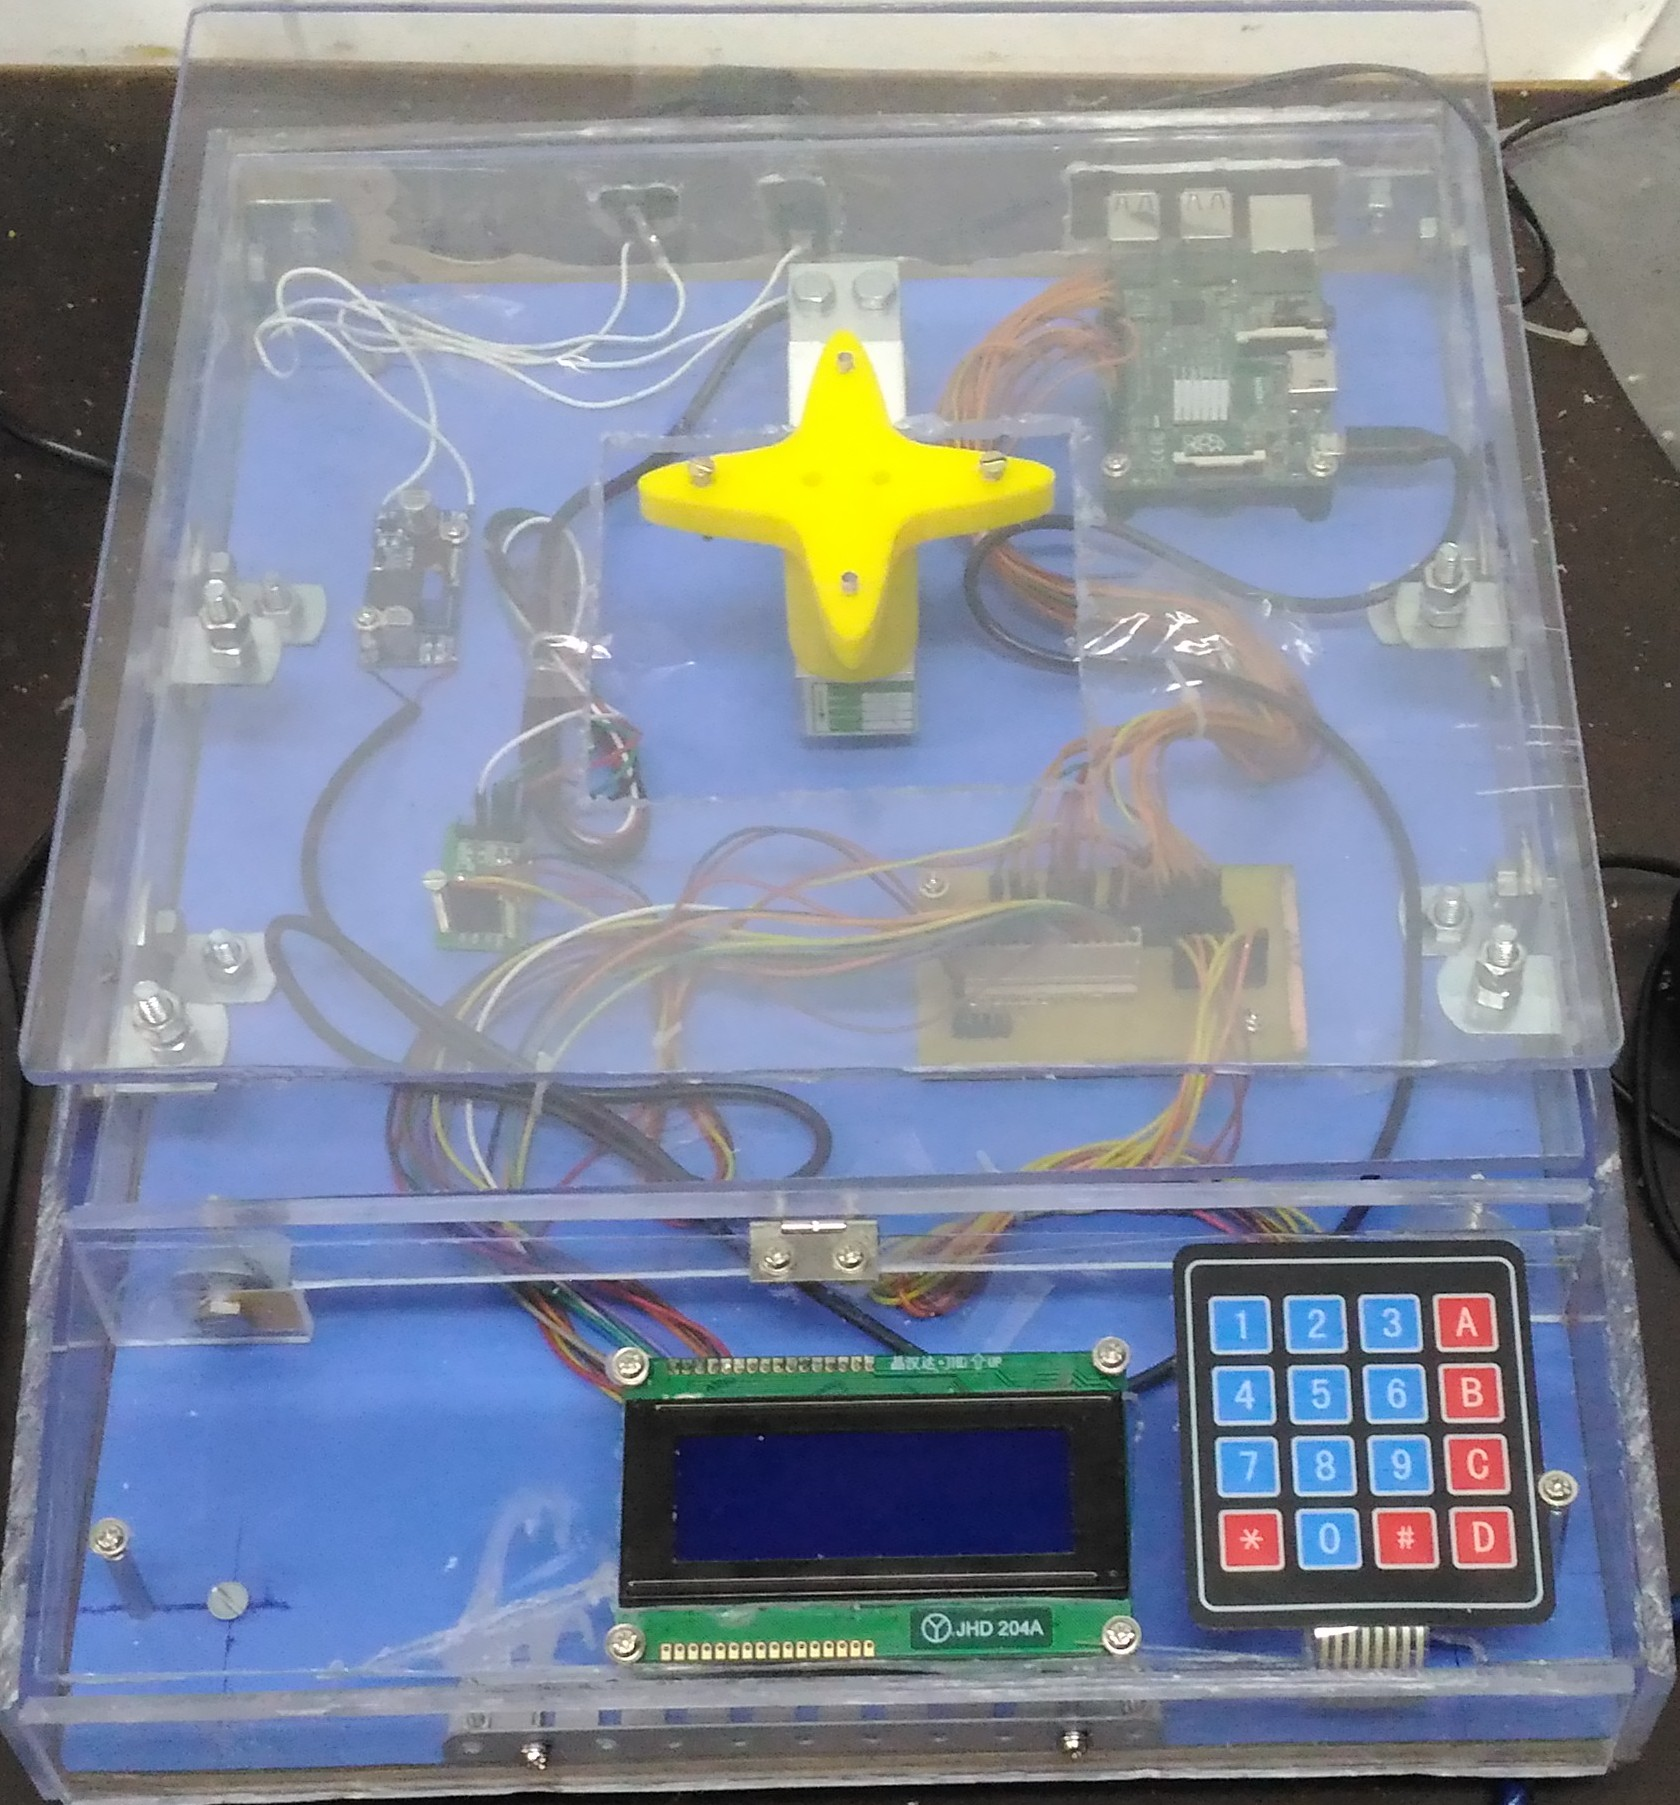
\includegraphics[width=7cm, height=7cm]{wm.jpg}

\section{Future Work}
In future this project can be made more effective by using image processing to identify which crop is put on the machine. We can also include bar-code or RFID module which will contain all the information about crop.\\
We can replace membrane keypad and LCD by touch screen.\\
This model can be transformed into more compact version.\\

\section{Bug Report And Challenges}
\begin{itemize}
\item Bug
\begin{itemize}
   \item Currently e-commerce website is unable to sent email to users using SMTP server.
   \item Two way handshaking between server and machine is not implemented yet. Although it is a rare situation, data might get lost some times while transferring it to server because tow way hand shaking is not implemented yet
\end{itemize}
\item Challenges
\begin{itemize}
   \item Building enclosure of weighing machine.
   \item Calibration of load cell.
   \item De-bouncing of keypad.
\end{itemize}
\end{itemize}
\begin{thebibliography}{li}
\bibitem{wavelan97} eyantra community\\
\bibitem{wavelan97} https://grabcad.com/library/keypad-4x4-membrane-1\\
\bibitem{wavelan97} http://www.tutorialspoint.com/python/python\_functions\\
\bibitem{wavelan97} http://www.tutorialspoint.com/python/python\_database\_access\\
\bibitem{wavelan97} https://grabcad.com/library/20x4-lcd-1\\
\bibitem{wavelan97} https://grabcad.com/library/raspberry-pi-model-b-2\\
\bibitem{wavelan97} http://forum.opencart.com/\\
\bibitem{wavelan97} http://stackoverflow.com/\\
\bibitem{wavelan97} https://sourceforge.net/p/raspberry-gpio-python/wiki/Inputs/\\
\bibitem{wavelan97} https://www.stewright.me/2014/06/tutorial-install-mysql-server-on-raspberry-pi/\\
\bibitem{wavelan97} https://pyformat.info/\\
\bibitem{wavelan97} http://mysql-python.sourceforge.net/MySQLdb.html\\
\bibitem{wavelan97} https://www.youtube.com/watch?v=nGUpzwEa4vg\\
\bibitem{wavelan97} https://www.youtube.com/watch?v=yYnX5QodqQ4\\
\bibitem{wavelan97} http://playground.arduino.cc/Learning/SoftwareDebounce\\
\bibitem{wavelan97} http://www.raspberrypi-spy.co.uk/2012/07/16x2-lcd-module-control-using-python/\\
\bibitem{wavelan97} http://code.stephenmorley.org/php/creating-downloadable-csv-files/\\
\bibitem{wavelan97} http://www.opencart.com/index.php?route=extension/extension/info\&extension\_id=24594\\
\end{thebibliography}

\end{document}


